\documentclass[sigconf,screen,review,natbib]{acmart}
\AtBeginDocument{%
\providecommand\BibTeX{{%
\normalfont B\kern-0.5em{\scshape i\kern-0.25em b}\kern-0.8em\TeX}}}

\setcopyright{acmcopyright}
\copyrightyear{2023}
\acmYear{2023}
\acmDOI{XXXXXXX.XXXXXXX}

\acmConference[PPDP '23]{25th International Symposium on
	Principles and Practice of Declarative Programming}{October 22--23,
	2023}{Cascais, Lisbon, Portugal}

\usepackage{amsmath}
\usepackage{multirow}
\usepackage{microtype}
\usepackage{tikz,tikz-qtree}
\usetikzlibrary{positioning}
\usetikzlibrary{arrows.meta, shapes.misc, positioning}
\usepackage{subfig}
\theoremstyle{definition}
\newtheorem{exmp}{Example}[section]
\usepackage[ruled, vlined, linesnumbered]{algorithm2e}
\SetKw{True}{true}
\SetKw{False}{false}
\SetKwInOut{Output}{Output}
\SetKwInOut{Input}{Input}
\SetKwData{typeInt}{Int}
\SetKwData{typeRat}{Rat}
\SetKwData{Defined}{Defined}
\SetKwFunction{parseStatement}{parseStatement}
\usepackage{libertine}

\title{A Differential Datalog Interpreter}

\author{Bruno Rucy Carneiro Alves de Lima}
\orcid{1234-5678-9012}
\affiliation{%
	\institution{University of Tartu}
	\department{Institute of Computer Science}
	\city{Tartu}
	\country{Estonia}
}
\email{bruno98@ut.ee}

\author{Merlin Kramer}
\affiliation{%
	\institution{unaffiliated}
	\city{Wuppertal}
	\country{Germany}
}
\email{merlin.kramer@gmail.com}

\author{Kalmer Apinis}
\affiliation{%
	\institution{University of Tartu}
	\department{Institute of Computer Science}
	\city{Tartu}
	\country{Estonia}
}
\email{kalmera@ut.ee}

\begin{abstract}
	The core reasoning task for datalog engines is materialization, the evaluation of a datalog program over
	a database alongside its physical incorporation into the database itself. The de-facto method of computing
	it, is through the recursive application of inference rules. Due to it being a costly operation, it is a must
	for datalog engines to provide incremental materialization, that is, to adjust the computation to new
	data, instead of restarting from scratch. One of the major caveats, is that deleting data is notoriously more
	involved than adding, since one has to take into account all possible data that has been entailed from what
	is being deleted. Differential Dataflow is a computational model that provides efficient incremental
	maintenance, notoriously with equal performance between additions and deletions, and work distribution, of
	iterative dataflows. In this paper we investigate the performance of materialization with three reference
	datalog implementations, out of which one is built on top of a lightweight relational engine, and the two others
	are differential-dataflow and non-differential versions of the same rewrite algorithm, with the same optimizations.
\end{abstract}

\keywords{datalog, incremental view maintenance, differential dataflow}

\begin{document}

\maketitle

\section{Introduction}
Datalog\cite{datalog}, the canonical language for reasoning over relational databases, ground fact stores, is a
declarative language used to evaluate sets of possibly-recursive restricted horn clauses, programs, while
remaining not Turing complete. Evaluating a program entails computing implicit consequences over a fact
store, yielding new facts.

Materialization, or the physical storage of a program's consequences, eliminates the need for reasoning
during query answering. Maintaining this computation is essential for modern Datalog use-cases, as it
relates to the broader problem of incremental view maintenance.

While the semi-naive evaluation method\cite{datalog} efficiently handles additions, deletions are often less efficient, as
retracting a fact may naively imply deleting all data derived from it. The delete-rederive\cite{dred} method addresses
this issue by computing the materialization adjustment through the generation of new Datalog programs, first
calculating all possible deletions, and then determining alternative derivations. The difference between these
sets represents the actual facts to be deleted.

However, using two distinct algorithms for additions and deletions results in different performance characteristics,
potentially causing severe biases. For example, when a large portion of ground facts are deleted, delete-rederive
could be significantly more expensive than re-materializing.

A promising way to tackle incremental maintenance in a more uniform manner is to use differential dataflow, a
programming model that efficiently processes and maintains large-scale possibly recursive dataflow computations. Central
to it is the notion of fine-grained tracking, with partially-ordered timestamps, and processing differences between
collections of data, rather than entire collections themselves. This approach facilitates efficient updates in response
to changes in the underlying data\cite{differential_dataflow}.

In the context of datalog, differential dataflow (DD) presents an opportunity to address the performance challenges
arising from handling additions and deletions. Contrary to traditional methods, such as semi-naive evaluation for
additions and delete-rederive for deletions, differential dataflow provides a unified and efficient approach to
incremental view maintenance.

The utilization of partially ordered timestamps and arrangements allows DD to precisely
identify affected parts of the computation and to recompute only the necessary components. This leads to
a more efficient handling of incremental updates in Datalog evaluation, as the system can focus on affected
sub-computations rather than re-evaluating the entire program. Furthermore, there also is first-class support
for both automatic parallelism and distributed computing, contributing to enhanced performance and scalability.

DDLog\cite{ddlog} has been the only attempt at building a datalog engine that utilized DD.
Similarly to the high-profile reasoner Souffle\cite{souffle}, it is a compiler, in which a datalog program
becomes an executable low-level language program, C++ in Souffle's case, and Rust for DDLog. The rationale for
the language choice, is that DD's canonical implementation lives as a heavily optimized
map-reduce-like framework written in Rust.

Notably, given that DDLog is a compiler, it is not suited for situations where either the program is expected
to be dynamic, with rules being added or removed, or where new programs ought to be evaluated during run
time, therefore restricting its use case to the specific scenarios where such drawbacks are acceptable.

There has been no study evaluating the isolated benefit of DD to datalog evaluation. Therefore
the suitability of DD in this context remains unclear, emphasizing the importance of further
research on its potential benefits and limitations in incremental view maintenance.

\textbf{Contributions.} In this work, we directly address the posited research question by developing a datalog
interpreter utilizing DD. We then compare our implementation with other prototypical datalog
interpreters, created from scratch, that share as many components as it is reasonable, in order to isolate
the effect of DD in both runtime performance and memory efficiency. This allows us to more
accurately empirically assess how does DD in itself fare against more traditional approaches.

Unlike DDLog, which compiles a datalog program into its evaluation as a fixed DD program, our
approach involves writing a single DD program capable of evaluating any datalog program. This
eliminates the need for compilation and provides the additional benefit of incremental maintenance for both rule
removals and additions.

\textbf{Structure of the paper.}
\begin{itemize}
	\item{\textbf{Background.}} A brief recapitulation of the general background, with datalog, its evaluation
	methods, and the delete-rederive method being formally introduced.
	\item{\textbf{Differential Evaluation.}} DD, and the translation of datalog evaluation to
	a dataflow is showcased and explained.
	\item{\textbf{System.}} The developed interpreters are described, alongside with all optimizations and
	benchmark-relevant information.
	\item{\textbf{Evaluation.}} An empirical evaluation of all reasoners, over multiple different programs and
	datasets is undertaken.
\end{itemize}
\section{Related Works}
\textbf{DD Applications and Related Projects.} There are two relevant DD projects that are worth
mentioning. One of them is Graspan, a parallel graph processing system that uses DD for efficient
incremental computation of static program analyses over large codebases.

Graspan models the program analysis problem as a reachability problem on a graph, where nodes represent program elements
and edges represent the relationships between these elements. It leverages DD to incrementally update
the analysis results in response to changes in the input graph, which can be due to code modifications or updates to
the analysis rules. Graspan has demonstrated its ability to scale to large codebases and provide low-latency updates
for various static analyses, including points-to analysis, control-flow analysis, and data-flow analysis.

Another project of interest is DBSP\cite{dbsp}, a recent development, that started from the need for a more concise
theoretical definition of DD. All of DBSP operators are based on DD's, however, its
computational model is less powerful as it does not allow updates to past values in a stream, and it is also assumed that
inputs arrive in time order. DBSP can express both incremental and non-incremental computations, with the former not being
possible in DD.

\textbf{Datalog engines.} There are two kinds of datalog engines. The first encompasses those that compile
a datalog program to usually a systems-level programming language, and the second are interpreters, able to
evaluate any datalog program.

Soufflé is a prominent example of a datalog compiler that translates datalog programs into high-performance
C++ code. It incorporates several optimization techniques, such as parallel execution with highly specialized data
structures\cite{souffle_btree}, and nearly optimal join ordering\cite{souffle_join}. Notably, its development has
been an unparalleled source of articles on the engineering of reasoners.

DDLog As previously mentioned, compiles datalog to DD, achieving efficient differential data updates
for datalog programs. It demonstrates the applicability of DD in the context of declarative logic
programming and incremental view maintenance.

The majority of reasoners recently developed have been mostly interpreters, further split into distributed or
shared memory systems. Out of the shared memory ones, the most notable are RDFox\cite{rdfox}, a highly specialized
and performant reasoner that is tailored to the semantic web needs, RecStep\cite{recstep}, that builds on top of a
highly efficient relational engine, and DCDatalog\cite{dcdatalog}, that builds upon the query optimizer DeALS\cite{deals}
and extends a work that establishes how some linear datalog programs could be evaluated in a lock-free manner, to
general positive programs.

One of the most high-profile datalog papers of interest has been BigDatalog\cite{bigdatalog}, that
originally used the query optimizer DeALs, and was built on top of the very popular Spark\cite{spark}
distribution framework. Soon after, a prototypical implementation\cite{cog} over Flink\cite{flink},
a distribution framework that supports streaming, Cog, followed. Flink, unlike Spark, supports
iteration, so implementing reasoning did not need to extend the core of the underlying framework. The most
successful attempt at creating a distributed implemention has been Nexus\cite{nexus}, that is also built on Flink,
and makes use of its most advanced feature, incremental stream processing.
\section{Background}
\textit{Datalog}\cite{datalog} is a declarative programming language. A program $P$ is a set of
rules $r$, with each $r$ being a restriction of tuple-generating dependencies: \[H(x_1, ..., x_j) \leftarrow \bigwedge_{i=1}^kB_i(x_1, ..., x_j) \]
with $k$, $j$ as finite integers, $x$ as terms, and each $B_i$ and $H$ as predicates. A term can belong
either to the set of variables, or constants. The set of all $B_i$ is called the \textit{body}, and $H$ the \textit{head}.

A rule $r$ is said to be datalog, if no predicate is negated, and all variables in the head appear somewhere in the body,
thereby not there being the possibility for existential variables to exist, conversely, a datalog program is one in which
all rules are datalog.
\begin{exmp}{Datalog Program}\label{ex1}
	\begin{align*}
		P = \{\text{SubClassOf}(?x, ?y) \leftarrow & \text{SubClassOf}(?x, ?y), \text{SubClassOf}(?y, ?z) \}
	\end{align*}
\end{exmp}
Example \ref{ex1} shows a simple valid recursive program. The single rule denotes that \textit{for all x, y, z, if x is
	in a SubClassOf relation with y, and y is in a SubClassOf relation with z, then it follows that x is in a subClassOf
	relation with z}.

Programs denote implications over a store of ground facts. This store is called the extensional database, $EDB$, and the result
of evaluating a program over some $EDB$ is the $IDB$, the intensional database.

Let $DB = EDB \cup IDB$, and for there to be a program $P$. We define the \textit{immediate consequence} of $P$ over $DB$ as
all facts that are either in $DB$, or stem from the result of applying the rules in $P$ to $DB$. The \textit{immediate consequence operator}
$\textbf{I}_C(DB)$ is the union of $DB$ and its immediate consequence, and the $IDB$, at the moment of the
application of $\textbf{I}_C(DB)$ is the difference of the union of all previous $DB$ with the $EDB$.

It is trivial to see that $I_C(DB)$ is monotone, and given that both the $EDB$ and $P$ are finite sets, and
that $IDB = \emptyset$ at the start, at some point $I_C(DB) = DB$, since there won't be new facts to be inferred. This
point is the \textit{least fixed point} of $I_c(DB)$\cite{datalog}. Computing the \textit{least fixed point} as
described, recursively applying the immediate consequence, is called Naive evaluation.
\subsection{Semi-Naive Evaluation}
The semi-naive evaluation algorithm \cite{datalog} is a widely-used technique for improving naive evaluation.
Given a Datalog program $P$ and an $EDB$, the algorithm iteratively computes the $IDB$ in the same manner as
naive evaluation, with the addition of maintaining a set of new delta facts $\Delta^+$ that are generated in
each iteration, that are utilized in a new delta program $\Delta^+P$.

Given a program $P$ with rules $r_0, ..., r_n$, with bodies $b(r) = \{b_0, ..., b_k\}$ and heads $h(r)$, the
delta program will generate one new $\Delta$rule for each $b_j$ in each rule body $b(r_i)$, in order to
represent that only facts that have been recently inferred are being taken into account.
\begin{exmp}{Semi-naive Evaluation Delta Program}
	\begin{align*}
		P = \{TC(?x, ?y) \leftarrow        & Edge(?x, ?y)                  \\
		TC(?x, ?z) \leftarrow              & TC(?x, ?y), TC(?y, ?z) \}     \\
		r_0 = TC(?x, ?y) \leftarrow        & Edge(?x, ?y)                  \\
		\Delta r_1 = TC(?x, ?z) \leftarrow & \Delta TC(?x, ?y), TC(?y, ?z) \\
		\Delta r_2 = TC(?x, ?z) \leftarrow & TC(?x, ?y), \Delta TC(?y, ?z)
	\end{align*}
	\label{exsne}
\end{exmp}
In theory, the semi-naive evaluation algorithm improves the efficiency of Datalog evaluation by avoiding
the recomputation of facts that have already been derived in previous iterations. This method is particularly
efficient for certain classes of Datalog programs that are common in practice. Example \ref{exsne} shows
the generated $\Delta$ program. It is worth noting, that there are substantial implementation challenges in order
to ensure that its overhead is not larger than the performance gains, since it possibly requires multiple
indexes and set operations to keep track of the most recently inferred facts, hence, it could be that in practice
naive evaluation might outperform it.

\subsection{Delete-Rederive}
Both the regular semi-naive and naive evaluation methods are already incremental, and easily handles the
addition of data. One merely has to continue the evaluation with all previous data as the most recent delta.

The most used method for handling deletions is a bottom-up algorithm\cite{dred} that uses semi-naive evaluation
to evaluate two new programs, one that computes all possible deletions that could stem from the deletion of the
facts being retracted, and then another that attempts to find alternative derivations to the overdeleted ones.

Given a program $P$ with rules $r_0, ..., r_n$, with bodies $b(r) = \{b_0, ..., b_k\}$ and heads $h(r)$, the
overdeletion program will generate one new $-$rule for each $b_j$ in each rule body $b(r_i)$, in order to represent
that if such fact were to be deleted, then $h(r_i)$ would not hold true.
\begin{exmp}{DRED Overdeletion Program}
	\begin{align*}
		P = \{TC(?x, ?y) \leftarrow   & Edge(?x, ?y)              \\
		TC(?x, ?z) \leftarrow         & TC(?x, ?y), TC(?y, ?z) \} \\
		-r_0 = -TC(?x, ?y) \leftarrow & -Edge(?x, ?y)             \\
		-r_1 = -TC(?x, ?z) \leftarrow & -Edge(?x, ?y), TC(?y, ?z) \\
		-r_2 = -TC(?x, ?z) \leftarrow & Edge(?x, ?y), -TC(?y, ?z)
	\end{align*}
	\label{ex6}
\end{exmp}
On example \ref{ex6} negative predicates represent overdeletion targets. For instance, if \verb|Edge(2, 3)| is
being deleted, then \verb|TC(2, 3)| will be deleted, and any other inferred fact that depends on it. Given that
it is a regular datalog program, it can be efficiently evaluated with semi-naive evaluation.

The next step is to compute the alternative derivations of the deleted facts, since some overdeleted facts might
still hold true. The alternative derivation program will generate one new $+$rule for each $r_i$ in $P$, with
one extra $-$ head predicate per body, representing an overdeleted fact. The $+$ program requires the overdeleted
facts to not be present.
\begin{exmp}{DRED Alternative Derivation Program}
	\begin{align*}
		P = \{TC(?x, ?y) \leftarrow  & Edge(?x, ?y)                          \\
		TC(?x, ?z) \leftarrow        & TC(?x, ?y), TC(?y, ?z) \}             \\
		r_0 = +TC(?x, ?y) \leftarrow & -TC(?x, ?y), Edge(?x, ?y)             \\
		r_1 = +TC(?x, ?z) \leftarrow & -TC(?x, ?z), Edge(?x, ?y), TC(?y, ?z)
	\end{align*}
	\label{ex7}
\end{exmp}
The output relations from example \ref{ex7} represent the data that has to be put back into the materialization.
The rationale for alternative derivations is that, for $r_1$, for instance, if the edge \verb|TC(3, 4)| was
overdeleted, because of there being \verb|Edge(1, 2)| and \verb|TC(2, 3)|, if \verb|Edge(3, 4)| was not deleted, by
rule $r_0$, then there is an alternative derivation for \verb|TC(3, 4)|.

As it can be seen, computing the maintenance of the materialization implies evaluating a program bigger than the
materialization itself, however, due to the fact that it is evaluated with semi-naive evaluation, the asymptotic
complexity remains the same. Nonetheless, in practice, deletion is often much slower than addition, as it can be
trivially seen by the worst-possible scenario, in which all facts are deleted, whereby while materialization would
be free, DRED would inquire an expensive overdeletion computation.

\subsection{Substitution-based evaluation}
The most impactful aspect of both of the introduced evaluation mechanisms is the implementation
of $I_c$ itself. The two most high-profile methods to do so are either purely evaluating the rules, or
rewriting them in some other imperative formalism, such as relational algebra, and executing it.

The substitution-based\cite{datalog} method is the simplest example of the former. A substitution $\sigma$ is
a homomorphism $[x_1 \rightarrow y_1, ..., x_i \rightarrow y_i]$, such that $x_i$ is a variable, and $y_i$ is
a constant. Given a not-ground fact, such as $TC(?x, 4)$, \textit{applying} the substitution $[?x \rightarrow 1]$ to
it will yield the ground fact $TC(1, 4)$.

Let $r$ be a Datalog rule of the form $h \leftarrow b_1, b_2, \ldots, b_m$, where $h$ is the head atom and $b_i$ are
the body atoms. Let $EDB$ be the set of ground facts for the input relations.

The substitution-based method computes the immediate consequence of the rule $r$ as follows:

Define the initial set of substitutions as $\Sigma_0 = \{ \sigma_0 \}$, where $\sigma_0$ is an empty substitution. For
each body atom $b_m$, find the set of ground facts $F_j \subseteq F$ that match $b_m$.

\begin{algorithm}
	\SetAlgoLined
	\Input{$\Sigma_{0}$, set of ground facts $F$, head atom $h$, body atom list $B$}
	\Output{Immediate Consequence $I$}
	\For{each $i = 1, 2, \ldots, m$}{
	\For{each fact $f \in F$ and each partial substitution $\sigma_{i-1} \in \Sigma_{i-1}$}{
	Generate an extension $\sigma'_{i-1}$ of $\sigma_{i-1}$ with the constant-to-variable homomorphisms from $f$ that are consistent with the current body atom $b_m$;

	\If{$\sigma'_{i-1}$ is a valid substitution)}{
	$\Sigma_i = \Sigma_{i - 1} \cup \sigma'_{i-1}$;
	}
	}
	\For{each final substitution $\sigma_m \in \Sigma_m$}{
		$I = I \cup \sigma_m{H}$
	}
	}
	\caption{Substitution-based Immediate Consequence}
\end{algorithm}
There is a noteworthy performance issue that arises due to the interaction between the substitution-based method
and DRED. During the alternate derivation phase, the new program has one more body atom. This can be prohibitively
more expensive to evaluate than the original program, since one extra body atom implies one extra iteration, which
could generate a polynomial number of substitutions, due to the cartesian product nature of each step.

\subsection{Relational algebra rewriting method}
Relational Algebra\cite{codd_1970} explicitly denotes operations over sets of tuples with fixed
arity, relations. It is the most popular database formalism that there is, with virtually every single
major database system adhering to the relational model\cite{pg,mysql,sqlserver} and using SQL as a
declarative syntax for relational algebra.

The translation of datalog rules to relational algebra equations is a well-known technique, and has been
the most successful strategy employed by the vast majority of all current state-of-the-art reasoners\cite{bigdatalog, cog, nexus, recstep, dcdatalog, souffle}
mostly due to the extensive industrial and academic research into developing data processing frameworks
that process very large amounts of data, and the techniques that have arisen from those.

Let $R$ and $T$ be relations with arity $r$ and $t$, $\theta$ be a binary operation with a boolean output, $R(i)$ be
the i-th column, all terms in the i-th position of every tuple in $R$, and $R[h, ..., k]$ be the subset of $R$ such
that only the columns $h, ..., k$ remain, and Const the set of all constant terms. The following are the most
relevant relational algebra operators and their semantics:
\begin{itemize}
	\item Selection by column $\sigma_{i=j)}(R) = \{ a \in R | a(i) == a(j) \}$
	\item Selection by value $\sigma_{i=k}(R) = \{a \in R | a(i) == k \}$
	\item Projection $\pi_{h, ..., k}(R) = \{(R(i), ..., R(j), \overrightarrow{C}) |  i, j >= 1 \wedge i, j <= r\ \wedge \forall c \in C. c \in \text{Const}$
	\item Product $\times(R, T) = \{(a, b) | a \in R \wedge b \in T \}$
	\item Join $\Join_{i=j} = \{(a, b) | a \in R \wedge b \in T \wedge a(i) == b(j)\}$
\end{itemize}
A relational algebra expression is in the $\mathcal{SPJ}$ form if it consists solely of select, project and join
operators. This form is very often seen in practice, being equivalent to \verb|SELECT ... FROM ... WHERE ...| SQL
queries, and highly benefits from being equivalent to conjunctive queries, that are equivalent to single-rule and
non-recursive datalog programs.

DD either implements, or makes it trivial to do so, all of the aforementioned relational algebra
operations, but lifted to the multiset domain, which implies that there must be some additional step to fit them
into datalog's set semantics.

\section{Differential Evaluation}
\subsection{Differential Dataflow} is a computational model that generalizes incremental processing to
times that are possibly partially ordered, and specifically operates over multisets of differences, which
can be either additions or retractions, instead of over the full data.

Let $C$ be a multiset, referred to as a collection, with $C_t$ being its value at a partially ordered
time $t$, and $C_t(b)$ being the unsigned integer representing weight of some record $b \in C_t$. We
establish that the difference of some collection $C$ at time $t$, named $\delta C_t$, is defined as: \[\delta C_t = C_t - C_{t - 1}\],
notably, differences can be both positive, representing additions, or negative, retractions, and it
also therefore holds that the value of $C_t$ can be reconstructed by the following equivalence: \[C_t = \sum_{i \leq t}\delta C_{i}\]

Let $A$ and $B$ be collections, and $\mathcal{OP}$ be some operator that maps a collection to some other
collection, or itself. Assuming $B$ to be the output of $\mathcal{OP}$ applied over $A$, computations in
DD follow the following: \[A_t = \sum_{i \leq t} \delta B_i = \mathcal{OP}(\sum_{i \leq t} \delta A_i)\]
with $\mathcal{OP}$ being proportional to $\delta A_t$, and not $A_t$.

Notably, a core premise of the canonical DD implementation, is in cleverly, and efficiently,
maintaining $\delta B$ and $\delta A$, specifically in the context of iterative dataflows, due to $t$ being
partially ordered.

Let's assume that a datalog program is being evaluated, and five fact updates, labeled as $\alpha_t$ arrive. In
regular semi-naive evaluation, even though rule application might happen in parallel, $\alpha_{t + 1}$ will only be
evaluated after $\alpha_{t}$ is, and the data used to compute each will always consist of all extensional and
intensional, previously inferred, facts.

In contrast, program evaluation could be written as a DD dataflow with two timestamps, $t$,
representing the time of arrival of the update, and $\langle a, b \rangle$, the product that keeps track of the
fixpoint evaluation, with $a$ being equal to $t$, and $b$ representing the current iteration count, respecting
the following partial order: \[\langle a_i, b_j \rangle \leq \langle c_k, d_l \rangle \iff a_i \leq c_k \wedge b_j \leq d_l\]

If we treat $\alpha_0$, $\alpha_1$, $\alpha_2$, $\alpha_3$ and $\alpha_4$ as differences with the following
respective timestamps: \[\langle 0, 0 \rangle, \langle 0, 1 \rangle, \langle 0, 2 \rangle, \langle 1, 1 \rangle, \langle 1, 2 \rangle\]
it is noticeable that $\alpha_1$ and $\alpha_4$ are comparable, but both of them, and vice-versa, are
incomparable with respect to $\alpha_2$ and $\alpha_3$. This, in turn, has two consequences in differential
dataflow. First, that the computation of both $\alpha_3$ and $\alpha_2$ happened independent of each other,
meaning both could have been computed in parallel, and, most importantly, that neither appeared in each other's
computation:
\begin{align*}
	\alpha_2 & = \delta A_{0, 2} = A_{0, 2} - (\delta A_{0, 0} + \delta A_{0, 1} )                  \\
	\alpha_3 & = \delta A_{1, 1} = A_{1, 1} - (\delta A_{0, 0} + \delta A_{0, 1} + \delta A_{1, 0})
\end{align*}
Within the context of datalog, the aforementioned evaluation semantics provide a full alternative to the way
incremental datalog evaluation is currently done, most specifically, the practical advantage of differential
dataflow, is that instead of using semi-naive evaluation and DRED, one can just describe the evaluation process
as a dataflow, and have both additions and deletions handled in the same way, with automatic parallelism and
distribution.
\subsection{Differential Substitution-based Method}
We now present a translation of algorithm I to DD, by emulating sequentially iterating over
each rule's body with relational joins, notably, all relational algebra operators are available through a map-
reduce-like API.
\begin{figure} [htb!]
	\centering
	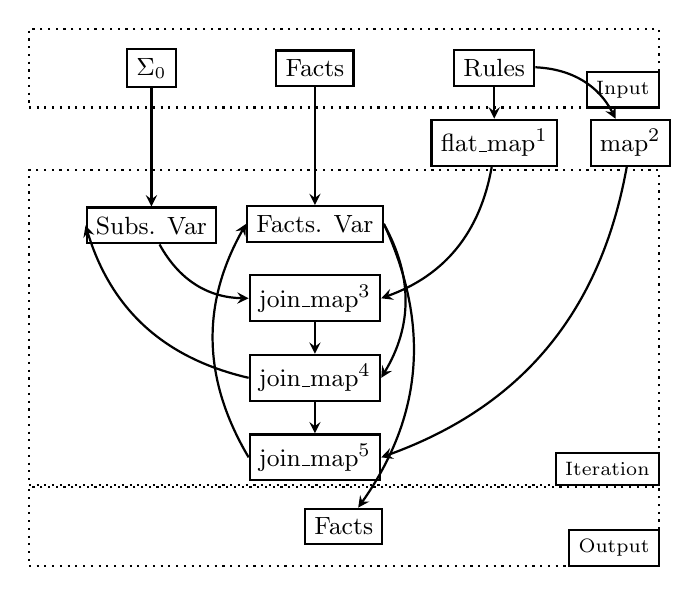
\begin{tikzpicture}[->,>=stealth,auto,node distance=6cm,
			thick,main node/.style={circle,draw,font=\sffamily\Large\bfseries}]

		%% Nodes
		\begin{scope}
			\node (inputs) at (0, 0) [draw, dotted, rectangle, minimum width=8cm, minimum height=1cm] {};
			\node (inputs_title) at (inputs.south east) [draw, anchor=south east] {\scriptsize Input};

			\node (blank) at (inputs.south) [minimum width=8cm, minimum height=1.5cm] {};

			\node (fixpoint) at (blank.south) [draw, dotted, rectangle, minimum width=8cm, minimum height=4cm, anchor=north] {};
			\node (fixpoint_title) at (fixpoint.south east) [draw, anchor=south east] {\scriptsize Iteration};

			\node (outputs) at (fixpoint.south) [draw, dotted, rectangle, minimum width=8cm, minimum height=1cm, anchor=north] {};
			\node (outputs_title) at (outputs.south east) [draw, anchor=south east] {\scriptsize Output};
		\end{scope}

		% Inputs
		\begin{scope}
			\node (empty_sub) [draw, right = 1.25cm of inputs.west] {\small $\Sigma_0$};
			\node (facts) [draw, right = 1.25cm of empty_sub.east] {\small Facts};
			\node (rules) [draw, right = 1.25cm of facts.east] {\small Rules};
		\end{scope}

		% No Iteration
		\begin{scope}
			\node (flat_map) at (blank) [draw, below = 4mm of rules] {$\text{\small flat\_map}^1$};
			\node (map) at (blank) [draw, right = 4mm of flat_map] {$\text{\small map}^2$};
		\end{scope}

		% Fixpoint Iteration

		\begin{scope}
			\node (subs_var) [draw, below = 15mm of empty_sub] {\small Subs. Var};
			\node (facts_var) at (fixpoint) [draw, below = 15mm of facts] {\small Facts. Var};
			\node (join1) at (fixpoint) [draw, below = 4mm of facts_var] {$\text{\small join\_map}^3$};
			\node (join2) at (fixpoint) [draw, below = 4mm of join1] {$\text{\small join\_map}^4$};
			\node (join3) at (fixpoint) [draw, below = 4mm of join2] {$\text{\small join\_map}^5$};
		\end{scope}

		% Outputs

		\begin{scope}
			\node (facts_output) at (outputs) [draw] {\small Facts};
		\end{scope}

		%% Edges
		\draw (facts) -- (facts_var);
		\path (facts_var.east) edge[bend left] (facts_output);
		\path (facts_var.east) edge[bend left] (join2.east);

		\draw (empty_sub) -- (subs_var);
		\path (subs_var) edge[bend right] (join1.west);
		\path (flat_map) edge[bend left] (join1.east);

		\draw (rules) -- (flat_map);
		\path (rules) edge[bend left] (map);

		\draw (join1) -- (join2);
		\path (join2.west) edge[bend left] (subs_var.west);
		\draw (join2) -- (join3);
		\path (join3.west) edge[bend left] (facts_var.west);
		\path (map) edge[bend left] (join3.east);
	\end{tikzpicture}
	\caption{Substitution method dataflow}
	\label{fig:substitution_simple_ddflow}
\end{figure}
Figure \ref{fig:substitution_simple_ddflow} depicts the substitution-based method as a dataflow. Superscripts denote
points of the dataflow that require further explanation. Furthermore, for clarity, we establish the shape of the
data, and the \verb|Var| suffix, that both facts and substitutions eventually take up. a Variable is used to express
recursive or iterative computations. It allows one to define iterative operations and data dependencies in the dataflow
graph, enabling the system to track and propagate changes across iterations efficiently, with product timestamps. Each
node either represents an operation, such as \verb|join_map|, that joins two streams and then applies a mapping function,
and \verb|flat_map|, that maps streams of iterables and then flattens them as a single stream.

We also note that this is a summarized description, with certain trivial, or too-implementation-oriented, parts
having had been omitted. $\Sigma_0$ is the stream of empty substitutions indexed per rule identifier, which will
be pre populated with one substitution, the empty one. We assume that rules have an unique identifier. Facts is
the relation-indexed stream of facts, and rules is the stream of rules, with two indexes, created with the operations
with superscripts $1$ and $2$.
\begin{enumerate}
	\item The first rule index indexes rules first by their identifier, and then by each of its body atoms, enumerating
	      them sequentially, imposing an order of evaluation as the original algorithm.
	\item The second rule index indexes by identifier and body size, being necessary to ensure that only the substitutions
	      which have been exhaustively expanded ought to be considered for application on the rule head.
	\item \verb|join_map| is an operator that joins two collections, and then applies a function. In this situation, the
	      function that is applied, is one that applies substitutions to the input atoms, therefore either creating new
	      atoms, with less variables as terms, or the very same ones. This is equivalent to the necessary setup for step 1
	      of Algorithm I to occur, making use of index $1$.
	\item The next join creates new substitutions, based on the newly minted atoms. All current substitutions are attempted
	      to be expanded further, with the ones being successful being emitted from the join.
	\item This is the last step of the algorithm, where all final substitutions are applied to the head of each rule, index
	      $2$, to then create new ground facts.
\end{enumerate}
\section{System}
In this section we provide a technical overview of the implemented reasoners, and what is shared between them, alongside
a novel indexing technique for the substitution-based method, that at the cost of increased memory usage, can significantly
decrease the number of times the operation that occurs the most frequently, substitution extension, occurs.

We name Chibi the reasoner that uses the substitution-based method without DD, and differential, the one
that does. Both of these reasoners share the implementation of the three core elements: unification, substitution application,
and in asserting that a fact is ground. All of the aforementioned operations are trivial, and each do not require more than
ten or so lines of code. Unification is a computationally cheap operation, given an atom, and a ground fact, the output is
a new substitution that maps the variables of the right to the constants of the left one, all others are self descriptive,
with substitution application merely substituting an atom's variables for the mapped variables in a substitution, and checking
if a fact is ground is done by ensuring that no terms are variables.

All three reasoners, Chibi, Differential and Relational, share the same simple in memory layout for the core elements of
datalog, and storage, notably, in Rust terms, it is to be assumed that all referred data structures are standard library
implementations, unless noted otherwise. Furthermore, a step of rule application is always done in parallel.
\begin{itemize}
	\item Constant: an enumeration of boolean, 64-bit integer or string, respectively named typed values.
	\item Variable: a 8 bit integer, hence imposing a bound on the number of variables that a rule can have
	\item Term: an enumeration of constant and variable
	\item Atom: A struct with a vector of terms, and a symbol, that can be either a 64-bit integer or a string
	\item Rule: A struct with an atom representing the head, and a vector of atoms as the body
	\item Storage: A Hash map of hash sets, with keys representing relation names, or id, and their respective
	      hash sets containing vectors of typed terms, ground facts.
\end{itemize}
Relational reasoner has one extra data structure, a btree index, that is used for sort-merge joins. Relational relies on
naively translating datalog rules into $\mathcal{SPJ}$, without any further optimizations whatsoever, aside from inserting
all data that is to be joined in its index, right before actually doing it. All relational operations and their evaluator
were implemented from scratch. The point of this reasoner is to evaluate how performant the popular relational algebra
evaluation can be in isolation, compared to the often forgotten substitution-based method, and differential.

Rule application until the least fixpoint is reached is done with semi-naive evaluation\cite{abiteboul}, with a program
transformation. DRED is implemented as described in \cite{dred}, in two steps, with both the overdeletion and alternative
derivation program being executed with semi-naive evaluation too. Both Chibi and Relational use the same function for this,
with differential evidently not using semi-naive evaluation neither DRED, given that it has its own iteration mechanism, as
demonstrated in figure \ref{fig:substitution_simple_ddflow}, and handling of additions and retractions.

\subsection{Demand-driven Multiple-column-based Indexing}
There is a possibly very large performance cost of the substitution-method, that can be exemplified in the specific scenario
of DRED, that could render it unable to be used in practice. As it was introduced, substitutions are both incrementally expanded,
and built anew, by iterating over every single body atom.

In the second step of DRED, an alternate derivation program is created. This program has one extra body atom, representing
overdeletions of the head's relation. This implies that this step could be prohibitively more expensive to evaluate than even
evaluating the program, due to the cartesian nature of the unification step, that implies iterating over the knowledge base once
once, for every atom. This inefficiency can be demonstrated the following example, in which the rule could be seen as the
alternate derivation step of some rule: $R(?x, ?z) <- T(?x, ?y), T(?y, ?z)$, with $-R$ representing the overdeletion estimation
from the previous step.

Let $P = \{+R(?x, ?z) \leftarrow -R(?x, ?z), T(?x, ?y), T(?y, ?z)\}$, and $EDB = \{T(a, b), T(b, c), T(c, d), -R(a, c), -R(b, d)\}$

Algorithm I will have three iterations:
\begin{enumerate}
	\item \begin{enumerate}
		      \item Current body atom: $-R(?x, ?z)$, $\Sigma_0$: $[\{\}]$
		      \item Fresh atoms - Applying all $\sigma : \Sigma_0$ to $-R(?x, ?z)$ yields $-R(?x, ?z)$
		      \item Substitution extension: \begin{enumerate}
			            \item unification: -R(?x, ?z) U -R(a, c) = $\{?x \rightarrow a, ?z \rightarrow c\}$
			            \item unification: -R(?x, ?z) U -R(b, d) = $\{?x \rightarrow b, ?z \rightarrow d\}$
		            \end{enumerate}
	      \end{enumerate}
	\item \begin{enumerate}
		      \item Current body atom: $T(?x, ?y)$, $\Sigma_1$: $[\{?x \rightarrow a, ?z \rightarrow c\}, \{?x \rightarrow b, ?z \rightarrow d\}]$
		      \item Fresh atoms - Applying all $\sigma : \Sigma_1$ to $T(?x, ?y)$ yields $T(a, ?z)$, $T(b, ?z)$
		      \item Substitution extension: \begin{enumerate}
			            \item unification: T(a, ?y) U T(a, b) = $\{?x \rightarrow a, ?y \rightarrow b, ?z \rightarrow c\}$
			            \item unification: T(a, ?y) U T(b, c) = none
			            \item unification: T(a, ?y) U T(c, d) = none
			            \item unification: T(b, ?y) U T(a, b) = none
			            \item unification: T(b, ?y) U T(b, c) = $\{?x \rightarrow b, ?y \rightarrow c, ?z \rightarrow d\}$
			            \item unification: T(b, ?y) U T(c, d) = none
		            \end{enumerate}
	      \end{enumerate}
	\item \begin{enumerate}
		      \item Current body atom: $T(?y, ?z)$, $\Sigma_2$: $[\{?x \rightarrow a, ?y \rightarrow b, ?z \rightarrow c\}, \{?x \rightarrow b, ?y \rightarrow c, ?z \rightarrow d\}]$
		      \item Fresh atoms - Applying all $\sigma : \Sigma_2$ to $T(?y, ?z)$ yields $T(b, c)$, $T(c, d)$
		      \item Substitution extension: \begin{enumerate}
			            \item unification: T(b, c) U T(a, b) = none
			            \item unification: T(b, c) U T(b, c) = $\{?x \rightarrow a, ?y \rightarrow b, ?z \rightarrow c\}$
			            \item unification: T(c, d) U T(c, d) = none
			            \item unification: T(c, d) U T(a, b) = none
			            \item unification: T(c, d) U T(b, c) = none
			            \item unification: T(c, d) U T(c, d) = $\{?x \rightarrow b, ?y \rightarrow c, ?z \rightarrow d\}$
		            \end{enumerate}
	      \end{enumerate}
\end{enumerate}
With the final substitutions being: $[\{?x \rightarrow a, ?y \rightarrow b, ?z \rightarrow c\}, \{?x \rightarrow b, ?y \rightarrow c, ?z \rightarrow d\}]$, therefore inferring two atoms:
$+R(a, c)$ and $+R(b, d)$. As it can be seen, the major source of inefficiency are the wasted calls to unification attempt, that could
grow polynomially with each new atom. The solution to this issue in theory is very straightforward; to avoid the cartesian product. We
devise a novel indexing technique specifically tailored to be portable to DD.

Returning to the example, it is trivial to see that unification attempts can be made optimal by joining on bindings; If $T(a, ?y)$ is the
left-hand side of unification, and $T(a, b)$, $T(b, c)$ are the candidates, no candidate that does not already match all constants
in $T(a, ?y)$ would produce a substitution extension. This significantly prunes the search space, to entirely avoid unifications that
would not yield substitution extensions.

We name our approach Demand-driven Multiple-column-based Indexing, because indexes are built on-demand to address the need of indices for
joining substitutions, that can be over multiple variables, therefore spanning over multiple columns, in each iteration. First, we demonstrate
the technique over the same example, and then provide a new version of Algorithm I, lastly, we modify the DD version to
also contain this indexing.
\begin{enumerate}
	\item \begin{enumerate}
		      \item Current body atom: $-R(?x, ?z)$, $\Sigma_0$: $[\{\}]$
		      \item Fresh atoms - Applying all $\sigma : \Sigma_0$ to $-R(?x, ?z)$ yields $-R(?x, ?z)$
		      \item Index 1 - Index all fresh atoms with the positions of their constant terms as keys: $\{[] : [[?x, ?z]]\}$
		      \item Index 2 - Index $-R$ based on all distinct values of the column keys of index 1 : $\{[]: [[a, c], [b, d]]\}$
		      \item Index 3 - Join Index 1 with Index 2:
		            \begin{enumerate}
			            \item $([?x, ?z], [[a, c]])$
			            \item $([?x, ?z], [[b, d]])$
		            \end{enumerate}
		      \item Attempt to unify:
		            \begin{enumerate}
			            \item unification: -R(?x, ?z) U -R(a, c) = $\{?x \rightarrow a, ?z \rightarrow c\}$
			            \item unification: -R(?x, ?z) U -R(b, d) = $\{?x \rightarrow b, ?z \rightarrow d\}$
		            \end{enumerate}
	      \end{enumerate}
	\item \begin{enumerate}
		      \item Current body atom: $T(?x, ?y)$, $\Sigma_1$: $[\{?x \rightarrow a, ?z \rightarrow c\}, \{?x \rightarrow b, ?z \rightarrow d\}]$
		      \item Fresh atoms - Applying all $\sigma : \Sigma_1$ to $T(?x, ?y)$ yields $T(a, ?y)$, $T(b, ?y)$
		      \item Index 1 - Index all fresh atoms with the positions of their constant terms as keys: $\{[0] : [[a, ?z], [b, ?z]]\}$
		      \item Index 2 - Index $T$ based on all distinct values of the column keys of index 1  $\{[0]: \{[a]: [[b]], [[b]]: [[c]], [c]: [[d]]\}\}$
		      \item Index 3 - Join Index 1 with Index 2:
		            \begin{enumerate}
			            \item $([?y], [[b]]])$
			            \item $([?y], [[c]]])$
		            \end{enumerate}
		      \item Attempt to unify:
		            \begin{enumerate}
			            \item unification: T(a, ?y) U T(a, b) = $\{?x \rightarrow a, ?y \rightarrow b, ?z \rightarrow c\}$
			            \item unification: T(b, ?y) U T(b, c) = $\{?x \rightarrow b, ?y \rightarrow c, ?z \rightarrow d\}$
		            \end{enumerate}
	      \end{enumerate}
	\item \begin{enumerate}
		      \item Current body atom: $T(?y, ?z)$, $\Sigma_2$: $[\{?x \rightarrow a, ?y \rightarrow b, ?z \rightarrow c\}, \{?x \rightarrow b, ?y \rightarrow c, ?z \rightarrow d\}]$
		      \item Fresh atoms - Applying all $\sigma : \Sigma_2$ to $T(?y, ?z)$ yields $T(b, c)$, $T(c, d)$
		      \item Index 1 - Index all fresh atoms with the positions of their constant terms as keys: $\{[0, 1] : [[b, c], [c, d]]\}$
		      \item Index 2 - Index $T$ based on all distinct values of the column keys of index 1 : $\{[0, 1]: \{[a, b]: [[]], [b, c]: [[]], [c, d]: [[]]\}\}$
		      \item Index 3 - Join Index 1 with Index 2:
		            \begin{enumerate}
			            \item $([b, c], [[]])$
			            \item $([c, d], [[]])$
		            \end{enumerate}
		      \item Attempt to unify:
		            \begin{enumerate}
			            \item unification: T(b, c) U T(b, c) = $\{?x \rightarrow a, ?y \rightarrow b, ?z \rightarrow c\}$
			            \item unification: T(c, d) U T(c, d) = $\{?x \rightarrow b, ?y \rightarrow c, ?z \rightarrow d\}$
		            \end{enumerate}
	      \end{enumerate}
\end{enumerate}
From this new example, it can be seen that the indexing scheme is relatively simple, relying on creating new indices that would allow unification
to never wastefully occur. We now structure it as Algorithm II.

Let $P : a \to [\mathbb{N}]$ be a function mapping an atom to an array of integers representing the positions of constants within the atom's terms, and
$R : ([\mathbb{N}], a) \to C$ another function, that maps an array of integers and an atom, to a subset of the atom's terms $c$ denoted by $C$.

The algorithm relies on two main indexes:
\begin{enumerate}
	\item $I_1 : P(a) \to 1^{\mathfrak{A}}$, where $1^{\mathfrak{A}}$ is the subset of
	      $\mathfrak{A}$ such that all $a$ have the same $P(a)$ value.
	\item $I_2 : P(a) \to I_3$, where $I_3 : R(F) \to 1^{F}$, and $1^{F}$ is the subset
	      of $F$ such that all $a$ have the same $R(P(a), a)$.
\end{enumerate}
\begin{algorithm}
	\SetAlgoLined
	\Input{$\Sigma_{0}$, set of ground facts $F$, head atom $H$, body atom list $B$}
	\Output{Immediate Consequence $I$}
	\For{each $i = 1, 2, \ldots, m$}{
	Apply $\Sigma_{i-1}$ to the current body atom to obtain fresh atoms $\mathfrak{A}$\;
	Create the first index $I_1 : P(a) \to 1^{\mathfrak{A}}$\;
	Create the second index $I_2 : P(a) \to I_3$\;
	Create the last index by joining Index 1 and Index 2: $I_4(a) = (I_1(a), I_2(a))$ for each $a \in \mathfrak{A}$\;
	\For{$(S_1, S_2) \in I_4$}{
	Unify each element in $S_1$ with each element in $S_2$\;

	Generate an extension $\sigma'_{i-1}$ of $\sigma_{i-1}$ with the constant-to-variable homomorphisms from $f$ that are consistent with the current body atom $b_m$;

	\If{$\sigma'_{i-1}$ is a valid substitution}{
	$\Sigma_i = \Sigma_{i - 1} \cup \sigma'_{i-1}$\;
	}
	}
	\For{each final substitution $\sigma_m \in \Sigma_m$}{
		$I = I \cup \sigma_m{H}$
	}
	}
	\caption{Substitution-based Immediate Consequence with Demand-driven Multiple-column-based Indexing}
\end{algorithm}
All indexing steps are $O(|F|)$ in time and data complexity, save for index two, that has worst-case data complexity of $O(|F| \cdot 2^{|a|}y)$, with $2^{|a|}$
representing the powerset of the number of terms in some atom $a$, and $F$ such that it has only atoms $a$. The product with the powerset arises due to how
indexing occurs by mapping all unique combinations of constant terms of fresh atoms, which in the worst-case could be exponential to arity.
\begin{figure}
	\centering
	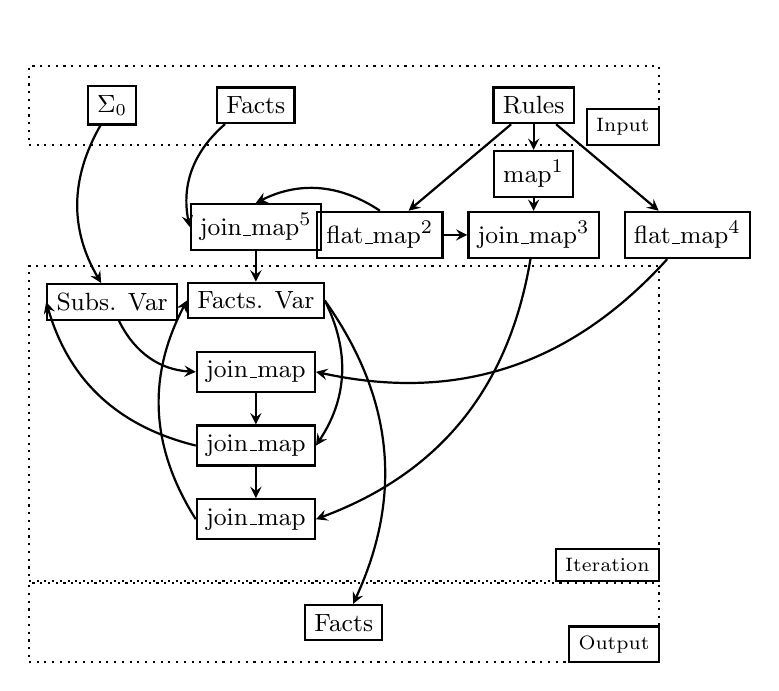
\begin{tikzpicture}[->,>=stealth,auto,node distance=6cm,
			thick,main node/.style={circle,draw,font=\sffamily\Large\bfseries}]
		%% Nodes
		\begin{scope}
			\node (inputs) at (0, 0) [draw, dotted, rectangle, minimum width=8cm, minimum height=1cm] {};
			\node (inputs_title) at (inputs.south east) [draw, anchor=south east] {\scriptsize Input};

			\node (blank) at (inputs.south) [minimum width=8cm, minimum height=3.0cm] {};

			\node (fixpoint) at (blank.south) [draw, dotted, rectangle, minimum width=8cm, minimum height=4cm, anchor=north] {};
			\node (fixpoint_title) at (fixpoint.south east) [draw, anchor=south east] {\scriptsize Iteration};

			\node (outputs) at (fixpoint.south) [draw, dotted, rectangle, minimum width=8cm, minimum height=1cm, anchor=north] {};
			\node (outputs_title) at (outputs.south east) [draw, anchor=south east] {\scriptsize Output};
		\end{scope}

		% Inputs
		\begin{scope}
			\node (empty_sub) [draw, right = 0.75cm of inputs.west] {\small $\Sigma_0$};
			\node (facts) [draw, right = 1cm of empty_sub.east] {\small Facts};
			\node (rules) [draw, right = 2.5cm of facts.east] {\small Rules};
		\end{scope}

		% No Iteration
		\begin{scope}
			\node (heads_ucc) at (blank) [draw, below = 11mm of rules] {$\text{\small join\_map}^3$};
			\node (ucc) at (blank) [draw, left = 3mm of heads_ucc] {$\text{\small flat\_map}^2$};
			\node (heads) at (blank) [draw, below = 3.25mm of rules] {$\text{\small map}^1$};
			\node (goals) at (blank) [draw, right = 3mm of heads_ucc] {$\text{\small flat\_map}^4$};
			\node (index) at (blank) [draw, below = 10mm of facts] {$\text{\small join\_map}^5$};
		\end{scope}

		% Fixpoint Iteration
		\begin{scope}
			\node (subs_var) [draw, below = 20mm of empty_sub] {\small Subs. Var};
			\node (facts_var) at (fixpoint) [draw, below = 20mm of facts] {\small Facts. Var};
			\node (join1) at (fixpoint) [draw, below = 4mm of facts_var] {$\text{\small join\_map}$};
			\node (join2) at (fixpoint) [draw, below = 4mm of join1] {$\text{\small join\_map}$};
			\node (join3) at (fixpoint) [draw, below = 4mm of join2] {$\text{\small join\_map}$};
		\end{scope}

		% Outputs

		\begin{scope}
			\node (facts_output) at (outputs) [draw] {\small Facts};
		\end{scope}

		%% Edges
		\path (facts) edge[bend right] (index.west);
		\path (facts_var.east) edge[bend left] (facts_output);
		\path (facts_var.east) edge[bend left] (join2.east);

		\path (empty_sub) edge[bend right] (subs_var);
		\path (subs_var) edge[bend right] (join1.west);

		\draw (rules) -- (ucc);
		\draw (rules) -- (heads);
		\draw (rules) -- (goals);
		\draw (ucc) -- (heads_ucc);
		\draw (heads) -- (heads_ucc);
		\path (ucc.north) edge[bend right] (index.north);
		\path (goals) edge[bend left] (join1.east);

		\draw (index) -- (facts_var);
		\draw (join1) -- (join2);
		\path (join2.west) edge[bend left] (subs_var.west);
		\draw (join2) -- (join3);
		\path (join3.west) edge[bend left] (facts_var.west);
		\path (heads_ucc) edge[bend left] (join3.east);
	\end{tikzpicture}
	\caption{Substitution method with indexing dataflow}
	\label{fig:substitution_indexed_ddflow}
\end{figure}
Figure \ref{fig:substitution_indexed_ddflow} displays the DD version of Algorithm II, that mostly remains exactly the same, save for
new operations happening during the phase before iteration. We now clarify the points of interest in the dataflow. There were no differences in the steps inside
iteration, aside from joins happening through the vector of constant positions and relation symbols,
instead of only relation symbols.
\begin{enumerate}
	\item The first \verb|map| operator remains the same, indexing rules by their identifier and body size, used to ensure
	      that only fully expanded substitutions will be applied to rule heads. The same as superscript $2$ in \ref{fig:substitution_simple_ddflow}.
	\item The unique column combinations of the input ruleset are computed by this operator. Unlike in the imperative description of the algorithm, where
	      column combinations are generated in each iteration, we pre generate all of them, and index them by relation symbol.
	\item This step joins the rule identifiers with the unique column combinations. This is only used at the very last join during iteration, to ensure that
	      the output fact is indexed by the correct column combination.
	\item Equivalent to superscript $1$ in \ref{fig:substitution_simple_ddflow}.
	\item With superscript $2$, the input fact stream can be immediately indexed by the necessary constant position combinations. This is done by a join on
	      relation symbol, that will index each fact by all column combinations.
\end{enumerate}
This dataflow is possibly much more efficient. An arrangement in DD is a pre-computed, indexed representation of a collection that allows
for efficient querying and manipulation of the data. These arrangements play a crucial role in optimizing the performance of dataflows. By carefully choosing
which arrangements to create and maintain, it is possible to minimize the computational overhead and reduce the need for expensive recomputations.

Most specifically, arrangements dictate the level of join parallelism, by the fact that the join operator shards the data among workers by the key of
the arrangement, partitioning the data to be joined by a more fine-grained key than relation symbol, such as relation symbol and positions occupied by constants,
constant values, as on Algorithm II, a higher degree of parallelism could be unlocked.
\section{Evaluation}
Three thorough experiments were conducted in order to showcase relative performance, scalability, and memory usage, of all reasoners, with the intent being twofold:
to evaluate the performance characteristics of DD, in isolation of virtually all other elements, and to establish as to whether general algorithmic
improvements, such as the demand-driven indexing scheme, are portable to DD.

\textbf{Setup.} The experiments were run on a google-cloud-provisioned x86 machine of type e2-standard-16, with 16 intel skylake cores and 64 gigabytes of RAM. Each
benchmark measurement was taken 70 times, with the 20 measurements of most variance removed, and averaged out.
% \begin{exmp}{RhoDFS inference rules}
% 	\begin{align*}
% 		T(?x, ?y, ?z) \leftarrow                 & rdf(?x, ?y, ?z)                \\
% 		T(?y, rdf:type, ?x) \leftarrow           & T(?a, rdfs:domain, ?x),        \\
% 		                                         & T(?y, ?a, ?z)                  \\
% 		T(?z, rdf:type, ?x) \leftarrow           & T(?a, rdfs:range, ?x),         \\
% 		                                         & T(?y, ?a, ?z)                  \\
% 		T(?x, rdfs:subPropertyOf, ?z) \leftarrow & T(?x, rdfs:subPropertyOf, ?y), \\
% 		                                         & T(?y, rdfs:subPropertyOf, ?z)  \\
% 		T(?x, rdfs:subClassOf, ?z) \leftarrow    & T(?x, rdfs:subClassOf, ?y),    \\
% 		                                         & T(?y, rdfs:subClassOf, ?z)     \\
% 		T(?z, rdf:type, ?y) \leftarrow           & T(?x, rdfs:subClassOf, ?y),    \\
% 		                                         & T(?z, rdf:type, ?x)            \\
% 		T(?x, ?b, ?y) \leftarrow                 & T(?a, rdfs:subPropertyOf, ?b), \\
% 		                                         & T(?x, ?a, ?y)
% 	\end{align*}
% 	\label{program:rhodfs}
% \end{exmp}
% \begin{exmp}{RhoDFS-s inference rules}
% 	\begin{align*}
% 		rdfs:domain(?a, ?x) \leftarrow        & rdf(?a, rdfs:domain, ?x)        \\
% 		rdfs:range(?a, ?x) \leftarrow         & rdf(?a, rdfs:range, ?x)         \\
% 		rdf:type(?y, ?x) \leftarrow           & rdf(?y, rdf:type, ?x)           \\
% 		rdfs:subPropertyOf(?x, ?z) \leftarrow & rdf(?x, rdfs:subPropertyOf, ?z) \\
% 		rdfs:subClassOf(?x, ?z) \leftarrow    & rdf(?x, rdfs:subClassOf, ?z)    \\
% 		rdf:type(?y, ?x) \leftarrow           & rdfs:domain(?a, ?x),            \\
% 		                                      & rdf(?y, ?a, ?z)                 \\
% 		rdf:type(?z, ?x) \leftarrow           & rdfs:range(?a, ?x),             \\
% 		                                      & rdf(?y, ?a, ?z)                 \\
% 		rdfs:subPropertyOf(?x, ?z) \leftarrow & rdfs:subPropertyOf(?x, ?y),     \\
% 		                                      & rdfs:subPropertyOf(?y, ?z)      \\
% 		rdfs:subClassOf(?x, ?z) \leftarrow    & rdfs:subClassOf(?x, ?y),        \\
% 		                                      & rdfs:subClassOf(?y, ?z)         \\
% 		rdf:type(?z, ?y) \leftarrow           & rdfs:subClassOf(?x, ?y),        \\
% 		                                      & rdf:type(?z, ?x)                \\
% 		rdf(?x, ?b, ?y) \leftarrow            & rdfs:subPropertyOf(?a, ?b),     \\
% 		                                      & T(?x, ?a, ?y)
% 	\end{align*}
% 	\label{program:rhodfss}
% \end{exmp}
\begin{table*}
	\caption{Dataset Overview}
	\begin{tabular}{|c|c|c|}
		\hline
		Dataset & Area of Interest & Programs                 \\
		\hline
		LUBM    & semantic web     & RhoDFS, RhoDFS-s, OWL2RL \\
		\hline
		RMAT1K  & synthetic        & tc                       \\
		\hline
		RAND1K  & synthetic        & tc                       \\
		\hline
	\end{tabular}
	\label{tab:datasets}
\end{table*}

\textbf{Datasets.} On table \ref{tab:datasets} all datasets and program names, or acronyms, are shown. There are two areas of interest. The semantic web has very
specific use-cases for datalog, and are the leading source of research in extending the datalog mathematical formalism, and in providing improvements to decades-old
algorithms, such as DRED, with the backward-forward algorithm\cite{dredbf}. Seeking ways to introduce tuple-generating dependencies to programs, with evaluation remaining
tractable, has been one of the most active research directions, with highly-influential papers establishing new families of datalog languages\cite{datalog_plus_minus} and
thoroughly exploring their complexity classes alongside even further extensions\cite{sticky,warded,monadic}. These advancements have been somewhat tested in practice, albeit
with no full reference implementation having been specified. The most comprehensive, and recent, is closed-source\cite{vadalog}. The leading datalog engine in general, is
also closed-source\cite{rdfox}, and is tailored specifically to the semantic web.

The second area of interest is of purely mathematical synthetic graph benchmarks, that allow for generating infinitely-scalable specific graph structures. all datasets however,
including LUBM\cite{lubm}, are synthetic, with the difference being that there are multiple specific programs for RhoDFS.
\begin{itemize}
	\item \textbf{LUBM} is a classic inference benchmark dataset for both RhoDFS and OWL2RL rulesets. The data is divided in two parts, the TBox, terminological box, that holds
	      an ontology able to describe universities, and the ABox, assertional box, that asserts facts about universities using the terminology in the TBox. The RhoDFS ruleset, depicted
	      on \ref{program:rhodfs}, is relatively simple, but complex, there being only a single relation that is mutually recursive in every single rule. RhoDFS-s \ref{program:rhodfss} is
	      an improved version of RhoDFS, that creates new relations for every single constant combination in the original program, avoiding every body atom implying a full dataset, mimicking
	      the relational selection. The last ruleset, OWL2RL, has over 100 rules and is by far the most complex, representing the lower bound of OWL2RL implications, specific of the LUBM
	      Tbox. More information on converting description logic entailments to datalog can be found on\cite{descr_to_dlog}.
	\item \textbf{RMAT1k}. is a graph generated by the \verb|rmat| profile of the GT\cite{gtgraph} graph generator, used to benchmark various other reasoners\cite{recstep}\cite{bigdatalog}.
	      The dataset is a graph with ten times the number of edges as vertices, that follows an inverse power-law distribution.
	\item \textbf{RAND1k} is also a graph generated with the \verb|rand| profile of GT. The dataset is comprised of a graph that has one thousand edges, with each
	      having 0.01 probability of being connected to every other. In spite of having a small number of nodes, it is incredibly dense, with the output of the transitive closure program having almost
	      a hundred times more edges than the initial graph.
\end{itemize}
\subsection{Runtime comparison}
\begin{table*}
	\caption{Runtime Experimental Results}
	\begin{center}
		\begin{tabular}{|c|c|c|c|c|c|c|c|c|c|c|c|c|c|c|c|c|c|}
			\hline
			Dataset & Program                 & Batch  & \multicolumn{3}{c|}{diff} & \multicolumn{3}{c|}{$\text{diff}^{I}$} & \multicolumn{3}{c|}{chibi} & \multicolumn{3}{c|}{$\text{chibi}^{I}$} & \multicolumn{3}{c|}{rel}                                                                       \\
			\hline
			        &                         &        & Mat                       & +                                      & -                          & Mat                                     & +                        & -    & Mat  & +    & -    & Mat  & +    & -    & Mat  & +    & -    \\
			\hline
			LUBM1   & \multirow{6}{*}{rdfs}   & 50\%   & 1.47                      & 1.43                                   & 1.40                       & 0.47                                    & 0.48                     & 0.49 & 124  & 530  & 584  & 0.84 & 1.13 & 1.62 & 0.71 & 1.02 & 1.58 \\
			        &                         & 75\%   & 2.15                      & 0.74                                   & 0.73                       & 0.67                                    & 0.29                     & 0.25 & 276  & 559  & 369  & 1.10 & 1.01 & 1.38 & 1.01 & 0.97 & 1.42 \\
			        &                         & 90\%   & 2.58                      & 0.33                                   & 0.34                       & 0.84                                    & 0.14                     & 0.13 & 397  & 573  & 168  & 1.40 & 1.02 & 1.22 & 1.26 & 1.03 & 1.42 \\
			        &                         & 99\%   & 2.91                      & 0.05                                   & 0.05                       & 0.95                                    & 0.05                     & 0.03 & 486  & 584  & 23   & 1.54 & 1.00 & 0.97 & 1.41 & 0.97 & 1.23 \\
			        &                         & 99.9\% & 2.94                      & 0.03                                   & 0.01                       & 0.97                                    & 0.03                     & 0.02 & 487  & 586  & 5.5  & 1.60 & 1.00 & 1.23 & 1.38 & 0.94 & 1.45 \\
			        &                         & 100\%  & 2.89                      & 0                                      & 0                          & 0.99                                    & 0                        & 0    & 487  & 0    & 0    & 1.34 & 0    & 0    & 1.20 & 0    & 0    \\
			\cline{2-18}
			        & \multirow{6}{*}{rdfs-s} & 50\%   & 0.84                      & 1.11                                   & 0.92                       & 0.27                                    & 0.29                     & 0.35 & 0.72 & 1.2  & 126  & 0.65 & 1.11 & 1.67 & 0.63 & 1.25 & 1.72 \\
			        &                         & 75\%   & 1.31                      & 0.46                                   & 0.49                       & 0.35                                    & 0.17                     & 0.16 & 1.11 & 1.04 & 103  & 1.11 & 1.21 & 1.3  & 0.94 & 1.03 & 1.41 \\
			        &                         & 90\%   & 1.67                      & 0.24                                   & 0.23                       & 0.40                                    & 0.09                     & 0.09 & 1.3  & 1.10 & 54   & 1.12 & 1.08 & 1.2  & 1.26 & 1.16 & 1.32 \\
			        &                         & 99\%   & 1.72                      & 0.05                                   & 0.05                       & 0.44                                    & 0.05                     & 0.02 & 1.5  & 1.1  & 9.5  & 1.48 & 1.09 & 1.1  & 1.28 & 1.20 & 1.58 \\
			        &                         & 99.9\% & 1.65                      & 0.03                                   & 0.02                       & 0.45                                    & 0.03                     & 0.02 & 1.5  & 1.0  & 2.9  & 1.39 & 1.10 & 1.0  & 1.46 & 1.32 & 1.52 \\
			        &                         & 100\%  & 1.77                      & 0                                      & 0                          & 0.45                                    & 0                        & 0    & 1.2  & 0    & 0    & 1.38 & 0    & 0    & 1.12 & 0    & 0    \\
			\cline{2-18}
			        & \multirow{6}{*}{owl2rl} & 50\%   & 3.16                      & 8.48                                   & 9.19                       & OOM                                     & OOM                      & OOM  & OOT  & OOT  & OOT  & 31.1 & 85.7 & 55.9 & 32.0 & 88.1 & 16.3 \\
			        &                         & 75\%   & 6.59                      & 4.91                                   & 5.00                       & OOM                                     & OOM                      & OOM  & OOT  & OOT  & OOT  & 66.8 & 71.7 & 36.4 & 85.1 & 81.3 & 16.1 \\
			        &                         & 90\%   & 9.50                      & 2.42                                   & 2.29                       & OOM                                     & OOM                      & OOM  & OOT  & OOT  & OOT  & 114  & 63.5 & 15.1 & 130  & 70   & 16.3 \\
			        &                         & 99\%   & 11.2                      & 0.04                                   & 0.03                       & OOM                                     & OOM                      & OOM  & OOT  & OOT  & OOT  & 114  & 60.2 & 2.52 & 156  & 34   & 0.60 \\
			        &                         & 99.9\% & 11.3                      & 0.03                                   & 0.02                       & OOM                                     & OOM                      & OOM  & OOT  & OOT  & OOT  & 117  & 73.3 & 1.3  & 161  & 34   & 0.61 \\
			        &                         & 100\%  & 11.2                      & 0                                      & 0                          & OOM                                     & 0                        & 0    & OOT  & 0    & 0    & 138  & 0    & 0    & 162  & 0    & 0    \\
			\hline
			RAND-1k & \multirow{6}{*}{tc}     & 50\%   & 0.06                      & 1.07                                   & 1.02                       & 0.03                                    & 0.08                     & 0.10 & 0.03 & 0.48 & 1.08 & 0.01 & 0.13 & 0.17 & 0.01 & 0.13 & 0.13 \\
			        &                         & 75\%   & 0.23                      & 0.94                                   & 0.91                       & 0.05                                    & 0.07                     & 0.07 & 0.14 & 0.42 & 2.25 & 0.02 & 0.12 & 0.23 & 0.02 & 0.13 & 0.16 \\
			        &                         & 90\%   & 0.64                      & 0.56                                   & 0.56                       & 0.07                                    & 0.06                     & 0.05 & 0.45 & 0.48 & 5.96 & 0.08 & 0.15 & 0.70 & 0.07 & 0.15 & 0.26 \\
			        &                         & 99\%   & 1.05                      & 0.17                                   & 0.17                       & 0.08                                    & 0.03                     & 0.03 & 0.77 & 0.52 & 0.72 & 0.12 & 0.16 & 0.15 & 0.11 & 0.16 & 0.16 \\
			        &                         & 99.9\% & 1.13                      & 0.03                                   & 0.03                       & 0.09                                    & 0.01                     & 0.01 & 0.85 & 0.43 & 0.11 & 0.16 & 0.07 & 0.06 & 0.14 & 0.05 & 0.05 \\
			        &                         & 100\%  & 1.15                      & 0                                      & 0                          & 0.10                                    & 0                        & 0    & 0.86 & 0    & 0    & 0.16 & 0    & 0    & 0.14 & 0    & 0    \\
			\hline
			RMAT-1k & \multirow{6}{*}{tc}     & 50\%   & 1.30                      & 13.0                                   & 11.2                       & 0.63                                    & 2.51                     & 3.83 & 0.99 & 5.01 & 7.70 & 0.12 & 1.40 & 2.03 & 0.20 & 1.36 & 1.72 \\
			        &                         & 75\%   & 5.29                      & 9.22                                   & 8.59                       & 1.51                                    & 2.13                     & 2.57 & 3.71 & 4.52 & 8.84 & 0.57 & 1.67 & 2.06 & 0.61 & 1.54 & 1.84 \\
			        &                         & 90\%   & 8.88                      & 4.09                                   & 3.91                       & 2.11                                    & 1.08                     & 0.95 & 6.17 & 5.25 & 9.48 & 0.89 & 1.72 & 2.11 & 0.89 & 1.67 & 2.01 \\
			        &                         & 99\%   & 12.0                      & 0.76                                   & 0.59                       & 2.40                                    & 0.06                     & 0.06 & 8.32 & 5.51 & 10.2 & 1.12 & 1.68 & 2.68 & 1.20 & 1.55 & 2.28 \\
			        &                         & 99.9\% & 12.7                      & 0.04                                   & 0.04                       & 2.36                                    & 0.01                     & 0.01 & 8.79 & 4.63 & 0.55 & 1.25 & 0.90 & 0.69 & 1.31 & 0.58 & 0.78 \\
			        &                         & 100\%  & 12.8                      & 0                                      & 0                          & 2.31                                    & 0                        & 0    & 8.78 & 0    & 0    & 1.26 & 0    & 0    & 1.30 & 0    & 0    \\
			\hline
		\end{tabular}
	\end{center}
	\label{tab:mainbenchmark}
\end{table*}
Table \ref{tab:mainbenchmark} pictures the main benchmark, in which three measurements, Mat, +, and -, for every batch size, are recorded. All measurements are in
\textbf{seconds}. If the batch size is 75\%, then Mat is the amount of time taken to materialize 75\% of the data, using regular semi-naive evaluation, + is how much
incremental materialization, of 25\% of the data, the remaining amount, also using semi-naive evaluation, took, and lastly, - is how much time DRED has taken to delete
the 25\% that has been added. This provides a comprehensive and thorough overview of the performance of DRED and semi-naive evaluation, compared to differential
dataflow, which offers an alternative to both.

Notably, the selection of facts in + and - can dramatically influence the performance of both DRED and DD. However, conducting extensive performance
estimations by running the algorithms on numerous random subsets of the data is impractical due to the extensive duration required to run the entire benchmark, coupled
with the factorial number of possible permutations. Thus, we chose to just select random subsets of the data that contained 50\%, 25\%, 10\%, 1\%, and 0.1\% of its
original size, as update sizes.

We discuss the table over each dataset and its respective programs. First, for LUBM under the rdfs program, all differential reasoners exhibit a clear trend of decreasing
update computation times, as the batch size increases, with $\text{diff}^{I}$ performing much better in general, up until updates get very small, possibly indicating
that at this level, indexing starts to have too big of an overhead. In the case of all other reasoners, the trend is very different, with all update times, curiously save for
chibi, which is orders of magnitude slower than all other reasoners,  not decreasing. This is unsurprising, due to the very strong degree of recursiveness of the
program, therefore showcasing that neither DRED nor semi-naive evaluation provide significant speedups over rematerialization, with the best result being for $\text{chibi}^I$, in
which updates and deletions, in spite of being constant, are up to 40\% faster.

All reasoners perform significantly better on rdfs-s, indicating the importance of the program. Chibi's pathological performance issue is entirely gone with the new program, and
its performance discrepancy with $\text{chibi}^{I}$ is almost eliminated, save for deletions, which remain several times slower than rematerialization.

In the most complex program, owl2rl, both chibi and diff are not able to finish materialization, with the former having had taken more than 1000 seconds, and the latter
exceeding 64 gigabytes of RAM. Differential performs in the same manner as the previous programs, with decreasing update times, and symmetry between additions and
deletions. Both $\text{chibi}^{I}$ and rel exhibit decreasing deletion reasoning times in aggressive cliffs, with little decrease for additions.

The transitive closure program is simple, and linear, therefore being embarassingly simple to incrementalize. For the RAND-1k dataset, differential reasoners once again
perform in the same manner, with incremental behavior scaling linearly with the size of the data. The same behavior is shown for all other reasoners, with a caveat, that
DRED only starts to be competitive once the update size is less than 10\% of the original data. For RMAT-1k, reasoning times are much longer, showcasing a significantly
more complex dataset, with all non-differential reasoners struggling to provide proportional update times save for update sizes of less than 1\%.

In sum, diff and $\text{diff}^{I}$ performed predictably irrespective of the dataset and program being run, always being faster, and having proportionally decreasing reasoning
times for updates, while at the same time being symmetric. All other reasoners did not show the expected incremental behavior, neither for semi-naive evaluation nor DRED unless
the update size was small, which is not necessarily a hindrance in practice, since rarely if ever a system will receive an update that is bigger than 10\% of the original size
of the data.
\subsection{Peak memory usage comparison.}
The results of the previous subsection cannot be seen in an entirely positive light without there being consideration for memory usage. DD relies on multiple
in-memory indexes to keep track of all changes, and as it was seen, it entirely failed a benchmark due to running out of memory, thus, in this section we analyze the results of
measuring peak memory usage over the previous experiments.
\begin{table*}
	\caption{Memory usage experimental results}
	\begin{center}
		\begin{tabular}{|c|c|c|c|c|c|c|}
			\hline
			Dataset                & Program & diff & $\text{diff}^{I}$ & chibi & $\text{chibi}^{I}$ & rel   \\
			\hline
			\multirow{3}{*}{LUBM1} & rdfs    & 488  & 466               & 631   & 941                & 722   \\
			                       & rdfs-s  & 495  & 383               & 573   & 665                & 579   \\
			                       & owl2rl  & 446  & OOM               & 42190 & 29269              & 25450 \\
			\cline{2-7}
			\hline
			RAND-1k                & tc      & 90   & 85                & 41    & 47                 & 31    \\
			\hline
			RMAT-1k                & tc      & 434  & 521               & 265   & 285                & 258   \\
			\hline
		\end{tabular}
	\end{center}
	\label{tab:memorybenchmark}
\end{table*}
Table \ref{tab:memorybenchmark} presents the peak memory usage for each of the methods and programs across different datasets. Memory usage is presented in megabytes. LUBM1
occupies 20 megabytes of disk space, RAND-1k and RMAT-1k, respectively, 100 kilobytes.

For LUBM1, with the 'rdfs' and 'rdfs-s' programs, all reasoners performed comparably with each other, with respect to memory usage, however, as seen on the previous table,
there are major differences in runtime performance between them, with the most extreme example being for chibi and $\text{diff}^{I}$, in which the former is over 1000x times
slower, while using almost 50\% more memory. Interestingly, diff performed significantly better for the owl2rl program, consuming 100 times less memory than chibi and rel. It
is likely that this is due to the aforementioned aggressive compaction mechanism by the in-memory LSM trees. Notably, the indexed version of diff, $\text{diff}^{I}$, ran out of
memory (OOM) for this program, indicating possible limitations of the indexing method for handling complex queries in large datasets, which conversely is not true in the case
of $\text{chibi}^{I}$, therefore being an issue with the DD implementation in itself.

In both the RAND-1k and RMAT-1k datasets, all differential reasoners consume at least twice as much memory as all other reasoners, while performing similarly for initial
materialization runtime. This posits an interesting counterpoint to the dominance in both memory usage and runtime shown with more complex programs. The reason for this
discrepancy, is that the TC program has a very large number of iterations, therefore causing a significantly greater flux in the dataflow, and since each iteration implies
a new difference being stored, memory usage can grow at a fast pace.

While there are major differences in runtime among all reasoners, with some being orders of magnitude faster, the same cannot be said about memory usage, which save for a
very large program, there are no clear winners, implying that the memory requirements for DD in itself are not greater than regular reasoners, save for
highly-iterative dataflows, and remains proportional to the computation. The starkest example of this is for the owl2rl program, which in spite of containing over a hundred
rules, does not output much more data than rdfs/rdfs-s.
\section{Conclusion}
In this article we introduced a novel datalog reasoner, with two different algorithms, whose core value proposition is in it using the promising, but relatively obscure,
DD model of computation, and evaluated it against two other reference implementations that shared as many components as reasonable. We also described an
indexing method that significantly sped up a often overlooked method of implementing reasoning, the substitution method, that was shown to have solved many pathological
performance issues in benchmarks, at very little cost of extra memory. In all experiments, all DD based reasoners implemented bested their non differential
counterparts, showing unparalleled scalability over increasing update sizes, alongside virtually no performance differences between additions and retraction, while remaining
competitive in memory usage. There are multiple ways in which the work could be expanded in the future, such as in porting it over to support negation and more expressive
variants of datalog, and most importantly, making it distributed, which DD provides out of the box.

\bibliographystyle{ACM-Reference-Format}
\bibliography{software}

\appendix

\section{Programs}
\begin{exmp}{RhoDFS inference rules}
	\begin{align*}
		T(?x, ?y, ?z) \leftarrow                 & rdf(?x, ?y, ?z)                \\
		T(?y, rdf:type, ?x) \leftarrow           & T(?a, rdfs:domain, ?x),        \\
		                                         & T(?y, ?a, ?z)                  \\
		T(?z, rdf:type, ?x) \leftarrow           & T(?a, rdfs:range, ?x),         \\
		                                         & T(?y, ?a, ?z)                  \\
		T(?x, rdfs:subPropertyOf, ?z) \leftarrow & T(?x, rdfs:subPropertyOf, ?y), \\
		                                         & T(?y, rdfs:subPropertyOf, ?z)  \\
		T(?x, rdfs:subClassOf, ?z) \leftarrow    & T(?x, rdfs:subClassOf, ?y),    \\
		                                         & T(?y, rdfs:subClassOf, ?z)     \\
		T(?z, rdf:type, ?y) \leftarrow           & T(?x, rdfs:subClassOf, ?y),    \\
		                                         & T(?z, rdf:type, ?x)            \\
		T(?x, ?b, ?y) \leftarrow                 & T(?a, rdfs:subPropertyOf, ?b), \\
		                                         & T(?x, ?a, ?y)
	\end{align*}
	\label{program:rhodfs}
\end{exmp}
\begin{exmp}{RhoDFS-s inference rules}
	\begin{align*}
		rdfs:domain(?a, ?x) \leftarrow        & rdf(?a, rdfs:domain, ?x)        \\
		rdfs:range(?a, ?x) \leftarrow         & rdf(?a, rdfs:range, ?x)         \\
		rdf:type(?y, ?x) \leftarrow           & rdf(?y, rdf:type, ?x)           \\
		rdfs:subPropertyOf(?x, ?z) \leftarrow & rdf(?x, rdfs:subPropertyOf, ?z) \\
		rdfs:subClassOf(?x, ?z) \leftarrow    & rdf(?x, rdfs:subClassOf, ?z)    \\
		rdf:type(?y, ?x) \leftarrow           & rdfs:domain(?a, ?x),            \\
		                                      & rdf(?y, ?a, ?z)                 \\
		rdf:type(?z, ?x) \leftarrow           & rdfs:range(?a, ?x),             \\
		                                      & rdf(?y, ?a, ?z)                 \\
		rdfs:subPropertyOf(?x, ?z) \leftarrow & rdfs:subPropertyOf(?x, ?y),     \\
		                                      & rdfs:subPropertyOf(?y, ?z)      \\
		rdfs:subClassOf(?x, ?z) \leftarrow    & rdfs:subClassOf(?x, ?y),        \\
		                                      & rdfs:subClassOf(?y, ?z)         \\
		rdf:type(?z, ?y) \leftarrow           & rdfs:subClassOf(?x, ?y),        \\
		                                      & rdf:type(?z, ?x)                \\
		rdf(?x, ?b, ?y) \leftarrow            & rdfs:subPropertyOf(?a, ?b),     \\
		                                      & T(?x, ?a, ?y)
	\end{align*}
	\label{program:rhodfss}
\end{exmp}

\end{document}
\endinput
%%% Local Variables:
%%% mode: latex
%%% TeX-master: t
%%% End:
